% ======================================================================
\section{Introduction}
\label{sec:intro}
% ======================================================================

\subsection{Why reduce dimension before learning?}

Turbulent and transitional flows are governed by partial differential equations
whose discretizations carry an enormous number of degrees of freedom. A direct
numerical simulation must resolve length scales from the integral scale down to
the Kolmogorov scale, and the number of grid points grows roughly as
$\mathrm{Re}^{9/4}$ for homogeneous turbulence \parencite{pope2000turbulent}.
Time-resolved particle image velocimetry (PIV) and large-eddy simulations of
engineering configurations likewise produce terabytes of spatio-temporal data.
Yet the dynamics recorded in these data are rarely as complex as their
dimension suggests. Coherent structures, symmetries, and dissipation confine
the long-time behavior of many flows to a comparatively thin subset of state
space. For dissipative systems this subset is sometimes formalized as an
\emph{inertial manifold} \parencite{foias1988inertial}, and more generally it
is the fluid-dynamical instance of the \emph{manifold hypothesis} that
underlies much of modern representation learning
\parencite{bengio2013representation,fefferman2016manifold}.

Dimensionality reduction (DR) exploits this structure by constructing a map
from the high-dimensional flow state to a small set of coordinates, and
usually also a map back. In fluid mechanics DR has served three overlapping
purposes. \emph{Analysis:} modal decompositions reveal coherent structures and
their frequencies \parencite{taira2017modal,taira2020modal}. \emph{Modeling:}
projection-based reduced-order models (ROMs) evolve a few modal amplitudes in
place of the full field \parencite{holmes2012turbulence,benner2015survey,rowley2017arfm}.
\emph{Learning:} most machine-learning (ML) models of fluid systems operate in a
compressed latent space because learning directly on the full state is
statistically and computationally prohibitive
\parencite{brunton2020ml,vinuesa2022enhancing,brunton2024promising}. This
review is concerned primarily with the third role, which inherits its
vocabulary and many of its tools from the first two.

The reasons to reduce dimension before learning are practical as well as
conceptual. Many-query tasks such as design optimization, uncertainty
quantification, control, and real-time simulation require thousands of
evaluations, which is exactly where surrogate models are valuable
\parencite{benner2015survey}. A learned model on a compact latent space has
fewer parameters, trains on far fewer samples, and can be rolled out
autoregressively at negligible cost. The latent coordinates can also be chosen
to make the downstream problem easier: approximately linear
\parencite{lusch2018koopman}, sparse in a function library
\parencite{champion2019sindyae}, statistically disentangled
\parencite{eivazi2022betavae,solera2024betavae}, or spatially local
\parencite{deshmukh2020dls,morton2026scitech}. The representation fixes an
upper bound on the fidelity of any model built on it. Features the encoder
discards cannot be recovered by the dynamics model, and features that are
represented in a tangled or temporally rough way make the forecasting problem
harder. Understanding the available DR techniques, and their consequences for
learning, is therefore a prerequisite for building reliable data-driven models
of fluid flows.

\subsection{Scope and relation to existing reviews}

Several excellent reviews cover parts of this landscape. Modal analysis of
fluid flows is surveyed by \textcite{taira2017modal,taira2020modal}, and the
theory of proper orthogonal decomposition (POD) by \textcite{berkooz1993} and
\textcite{holmes2012turbulence}, and textbook treatments of data-driven
modeling and reduced-basis methods are given by \textcite{brunton2019data} and
\textcite{hesthaven2016certified}. Projection-based model reduction is reviewed by
\textcite{benner2015survey}, \textcite{rowley2017arfm},
\textcite{lassila2014mor}, and \textcite{hesthaven2022acta}, and intrusive and
non-intrusive ROMs are surveyed briefly by \textcite{padula2024brief}. Closure modeling
is reviewed by \textcite{ahmed2021closures}. Machine learning for fluid
mechanics more broadly is reviewed by \textcite{brunton2020ml},
\textcite{duraisamy2019turbulence}, \textcite{vinuesa2022enhancing},
\textcite{vinuesa2024perspectives}, and \textcite{brunton2024promising}.
Operator inference is reviewed by \textcite{kramer2024opinf}. Closest in
spirit to the present article is the tutorial of \textcite{mendez2023linear},
which connects linear and nonlinear DR from fluid mechanics to ML, together
with the comparative study of \textcite{csala2022comparing}.

The present review differs in three ways. First, it is organized around the
\emph{use} of reduced coordinates in learning pipelines, so it treats encoder
design and latent dynamics jointly and emphasizes the properties of a latent
space that matter for forecasting. Second, it gives explicit attention to
\emph{spatially localized} representations, from domain-decomposed reduced
bases to generalized finite element enrichment and data-informed local
subspaces (DLS) \parencite{deshmukh2020dls}. These have received less attention
in the ML literature than global modal and autoencoder bases, yet they address
directly the multi-scale character of high-Reynolds-number turbulence. Third,
it includes computed examples that make the central trade-offs concrete: the
Kolmogorov $n$-width of transport problems, the accuracy ceiling of learned
nonlinear decoders, and the effect of localization on a turbulent cavity flow.
We restrict attention to reduction of the \emph{state} (the flow field). Sensor
placement, super-resolution, and closure modeling are mentioned only where they
bear directly on representation.

\subsection{Organization}

\Cref{fig:timeline} places the methods discussed here on a common timeline,
grouped into five families that also structure the article.
\Cref{sec:formulation} introduces notation, defines what is meant by a good
reduced representation, and presents a taxonomy.
\Cref{sec:linear} reviews linear subspace methods and their limitations, and
\cref{sec:local} reviews sparse, clustered, and spatially localized
representations, including DLS. \Cref{sec:manifold} covers classical
(non-neural) manifold learning, and \cref{sec:autoencoders} covers neural
autoencoders. \Cref{sec:meshfree} discusses graph-based, mesh-agnostic, and
operator-learning representations. \Cref{sec:dynamics} examines how reduced
coordinates are coupled to learned dynamics. \Cref{sec:assessment} provides a
comparative assessment with recommendations on baselines and metrics, and
\cref{sec:outlook} outlines open challenges.

\begin{figure}[tbp]
  \centering
  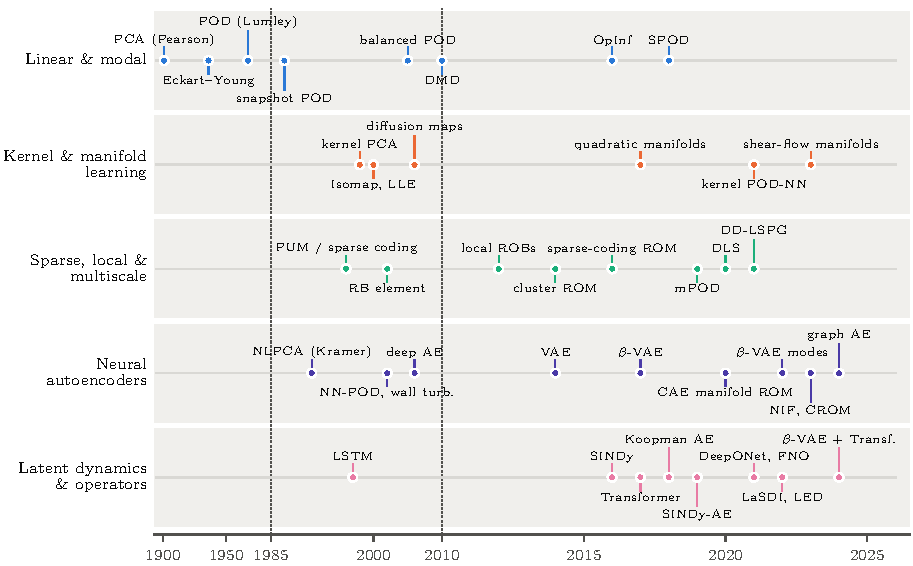
\includegraphics[width=\textwidth]{figs/timeline.pdf}
  \caption{Selected developments in dimensionality reduction relevant to fluid
  dynamics, grouped by family. The time axis is piecewise linear, with changes
  of scale at 1985 and 2010 (dashed lines). Representative references:
  PCA \parencite{pearson1901}, Eckart--Young \parencite{eckart1936},
  POD \parencite{lumley1967}, snapshot POD \parencite{sirovich1987},
  balanced POD \parencite{rowley2005bpod}, DMD \parencite{schmid2010dmd},
  OpInf \parencite{peherstorfer2016opinf}, SPOD \parencite{towne2018spod};
  kernel PCA \parencite{scholkopf1998kpca}, Isomap and LLE
  \parencite{tenenbaum2000isomap,roweis2000lle}, diffusion maps
  \parencite{coifman2006diffusion}, quadratic manifolds
  \parencite{jain2017quadratic}, kernel POD--NN \parencite{salvador2021kpod},
  shear-flow manifolds \parencite{farzamnik2023snapshots};
  PUM and sparse coding \parencite{melenk1996pum,olshausen1996},
  RB element \parencite{maday2002rbe}, local ROBs \parencite{amsallem2012local},
  cluster ROM \parencite{kaiser2014cluster}, sparse-coding ROM
  \parencite{deshmukh2016sparse}, mPOD \parencite{mendez2019mpod},
  DLS \parencite{deshmukh2020dls}, DD-LSPG \parencite{hoang2021ddlspg};
  NLPCA \parencite{kramer1991nlpca}, NN-POD for wall turbulence
  \parencite{milano2002}, deep AE \parencite{hinton2006reducing},
  VAE \parencite{kingma2014vae}, $\beta$-VAE \parencite{higgins2017betavae},
  CAE manifold ROM \parencite{lee2020cae}, $\beta$-VAE modes
  \parencite{eivazi2022betavae}, NIF and CROM \parencite{pan2023nif,chen2023crom},
  graph AE \parencite{pichi2024gca};
  LSTM \parencite{hochreiter1997lstm}, SINDy \parencite{brunton2016sindy},
  Transformer \parencite{vaswani2017attention}, Koopman AE
  \parencite{lusch2018koopman}, SINDy-AE \parencite{champion2019sindyae},
  DeepONet and FNO \parencite{lu2021deeponet,li2021fno}, LaSDI and LED
  \parencite{fries2022lasdi,vlachas2022led}, and $\beta$-VAE with transformer
  \parencite{solera2024betavae}.}
  \label{fig:timeline}
\end{figure}
